\documentclass[letterpaper]{book}
\PassOptionsToPackage{usenames,dvipsnames,svgnames,table,xcdraw}{xcolor}
\PassOptionsToPackage{dvipsnames,svgnames,table,xcdraw}{enumitems}


%**************************************************************
%References for commands and symbols:
%1. https://en.wikibooks.org/wiki/LaTeX/Mathematics
%2. http://latex.wikia.com/wiki/List_of_LaTeX_symbols
%**************************************************************
\usepackage{yfonts}

\usepackage{array}
\usepackage{scalerel}
\usepackage{setspace}
%\usepackage{amsmath
%\usepackage{amssymb}
% \usepackage{amsbsy}
\usepackage{amsfonts}
\usepackage{mathtools} 
\usepackage{bm}
\usepackage{upgreek}

\usepackage{relsize} % for larger math symbols


\usepackage{adjustbox}
\usepackage{tikz}
\usetikzlibrary{arrows, matrix}
\usepackage[siunitx]{circuitikz}
\usetikzlibrary{calc,patterns,decorations.pathmorphing,decorations.markings,arrows.meta, positioning}

\usepackage{pgfplots}
\pgfplotsset{compat=newest}

\usepackage{empheq}

% \usepackage{bbm}
% \usepackage{bbold}
\let\proof\relax 
\let\endproof\relax
\usepackage[cm]{fullpage}
\usepackage{tocloft}

\usepackage{float}
\usepackage{alltt}

\usepackage{placeins}

\usepackage{url}
\usepackage[utf8]{inputenc} % for boxes
\usepackage[T1]{fontenc}
\usepackage{lmodern}
\usepackage{minted}         % For code highlighting
% Optional: To globally set line breaks and frame for minted code blocks
\setminted[julia]{
    frame=single,
    breaklines=true,
    fontsize=\footnotesize,
    linenos
}


\usepackage{pdfpages}
\usepackage{enumerate}
\usepackage[most]{tcolorbox}
\tcbuselibrary{theorems}

\usepackage{siunitx}

%\usepackage{booktabs} % for better table formatting

\usepackage{MnSymbol}

\usepackage{mathdots}
\usepackage{xfrac}
\usepackage{fix-cm} % Fixes warnings about missing fonts; see http://tex.stackexchange.com/questions/32378/xfrac-siunitx-gives-me-a-font-warning


% Font Settings
\usepackage{avant} % Use the Avantgarde font for headings
%\usepackage{mathptmx} % Use the Adobe Times Roman as the default text font together with math symbols from the Sym­bol, Chancery and Com­puter Modern fonts

\usepackage{subcaption}
%\usepackage{subfig}
\usepackage{graphicx} 
\graphicspath{{graphics/}}
%\usepackage[T1]{fontenc}
%\usepackage[usenames,dvipsnames,svgnames,table, xcdraw]{xcolor}
%\usepackage[caption=false,font=footnotesize]{subfig}
%\usepackage[utf8]{inputenc}
%\usepackage{bmpsize}
% \usepackage{caption}
% \captionsetup{size=footnotesize,
%     %justification=centering, %% not needed
%     skip=5pt, position = bottom}
% \let\proof\relax 
% \let\endproof\relax
\usepackage{amsthm}
%\usepackage{algorithm}
\usepackage{algorithmicx}
%\usepackage{algpseudocode}
\usepackage{mathrsfs}
\usepackage[ruled,vlined]{algorithm2e}
\usepackage{times}
\usepackage{multicol}
%\usepackage[caption=false,font=footnotesize]{subfig}
%\usepackage[utf8]{inputenc}
\usepackage[T1]{fontenc}
\usepackage{textcomp}
\usepackage{balance}
%\usepackage[sort,numbers]{natbib}
\usepackage{multirow}
\usepackage{booktabs}
%\usepackage{dblfloatfix} 

\usepackage{makecell}
\usepackage{hhline} % double-line in a table
%\usepackage[]{hyperref}
\usepackage[colorlinks]{hyperref}
\definecolor{BrickRed}{rgb}{0.7,0.15,0.15}
\hypersetup{colorlinks=true,pdfpagemode=UseNone,citecolor=black,linkcolor=black,urlcolor=BrickRed}

\definecolor{mylightblue}{rgb}{0.8,0.9,1}
\usepackage{comment}
\usepackage{stackengine}

\usepackage{xparse}
\usepackage{lipsum}
%\usepackage{subcaption}
\usepackage{soul} 
\usepackage{times}
%\usepackage{cite} % to group references
%\usepackage[usenames,dvipsnames,svgnames,table,xcdraw]{xcolor}
%\usepackage[dvipsnames,svgnames,table,xcdraw]{xcolor}
\definecolor{shadecolor}{rgb}{0.9,0.9,0.9}
% \usepackage[sort, numbers]{natbib}
%\usepackage{balance}
\usepackage{enumitem}

\usepackage{mdframed}
\usepackage{framed}

\usepackage{listings}

\lstset{literate=
  {á}{{\'a}}1 {é}{{\'e}}1 {í}{{\'i}}1 {ó}{{\'o}}1 {ú}{{\'u}}1
  {Á}{{\'A}}1 {É}{{\'E}}1 {Í}{{\'I}}1 {Ó}{{\'O}}1 {Ú}{{\'U}}1
  {à}{{\`a}}1 {è}{{\`e}}1 {ì}{{\`i}}1 {ò}{{\`o}}1 {ù}{{\`u}}1
  {À}{{\`A}}1 {È}{{\'E}}1 {Ì}{{\`I}}1 {Ò}{{\`O}}1 {Ù}{{\`U}}1
  {ä}{{\"a}}1 {ë}{{\"e}}1 {ï}{{\"i}}1 {ö}{{\"o}}1 {ü}{{\"u}}1
  {Ä}{{\"A}}1 {Ë}{{\"E}}1 {Ï}{{\"I}}1 {Ö}{{\"O}}1 {Ü}{{\"U}}1
  {â}{{\^a}}1 {ê}{{\^e}}1 {î}{{\^i}}1 {ô}{{\^o}}1 {û}{{\^u}}1
  {Â}{{\^A}}1 {Ê}{{\^E}}1 {Î}{{\^I}}1 {Ô}{{\^O}}1 {Û}{{\^U}}1
  {Ã}{{\~A}}1 {ã}{{\~a}}1 {Õ}{{\~O}}1 {õ}{{\~o}}1
  {œ}{{\oe}}1 {Œ}{{\OE}}1 {æ}{{\ae}}1 {Æ}{{\AE}}1 {ß}{{\ss}}1
  {ű}{{\H{u}}}1 {Ű}{{\H{U}}}1 {ő}{{\H{o}}}1 {Ő}{{\H{O}}}1
  {ç}{{\c c}}1 {Ç}{{\c C}}1 {ø}{{\o}}1 {å}{{\r a}}1 {Å}{{\r A}}1
  {€}{{\euro}}1 {£}{{\pounds}}1 {«}{{\guillemotleft}}1
  {»}{{\guillemotright}}1 {ñ}{{\~n}}1 {Ñ}{{\~N}}1 {¿}{{?`}}1
}

% \usepackage[utf8]{inputenc}
% \usepackage[T1]{fontenc}
% \usepackage{minted}


\definecolor{codegreen}{rgb}{0,0.6,0}
\definecolor{codegray}{rgb}{0.5,0.5,0.5}
\definecolor{codepurple}{rgb}{0.58,0,0.82}
\definecolor{backcolour}{rgb}{0.95,0.95,0.92}

\lstdefinestyle{mystyle}{
    backgroundcolor=\color{backcolour},   
    commentstyle=\color{codegreen},
    keywordstyle=\color{magenta},
    numberstyle=\tiny\color{black},
    stringstyle=\color{black},
    basicstyle=\ttfamily\normal,
    breakatwhitespace=false,         
    breaklines=true,                 
    captionpos=b,                    
    keepspaces=true,                 
    numbers=left,                    
    numbersep=5pt,                  
    showspaces=false,                
    showstringspaces=false,
    showtabs=false,                  
    tabsize=2
}
\lstset{style=mystyle}


\usepackage{mathtools}
\usepackage[english]{babel}
%\usepackage{minted}

\makeatletter
% \usepackage{tikz}
% \usetikzlibrary{calc}
% \newcommand*\circled[1]{\tikz[baseline=(char.base)]{
%     \node[shape=circle, draw, inner sep=1pt, 
%         minimum height={\f@size*1.6},] (char) {\vphantom{WAH1g}#1};}}
\makeatother

\usepackage{placeins}

\newcommand{\rb}[1]{\raisebox{1.5ex}{#1}}
 \newcommand{\trace}{\mathrm{trace}}



%\def\real{\mathbb{R}}
\newcommand{\real}{\mathbb R}
\def\reals{\mathbb{R}} %????
\newcommand{\nat}{\mathbb N}   
\newcommand{\whole}{\mathbb Z}    
\newcommand{\cp}{\mathbb C}    
\newcommand{\rat}{\mathbb Q} 
\newcommand{\im}{\mathbb i}
\newcommand{\impart}[1]{\mathrm{imag} \left( #1 \right)}
\newcommand{\repart}[1]{\mathrm{real} \left( #1 \right)}
%\newcommand{\angle}[1]{\mathrm{angle} (#1 )}

% Hack for a bold integral sign
\newcommand{\boldint}{%
    \ThisStyle{%
        \setbox0=\hbox{$\SavedStyle\int$}%
        \ooalign{%
            \hfil\scalebox{1.05}[1]{$\SavedStyle\int$}\hfil\cr
            \hfil\scalebox{1.1}[1]{$\SavedStyle\int$}\hfil\cr
            \hfil\scalebox{1.15}[1]{$\SavedStyle\int$}\hfil\cr
        }%
    }%
}
\newcommand{\customdot}[1]{\stackon[1.5pt]{$#1$}{\tiny\textbullet}}



\newcommand{\ds}{\displaystyle}
\newcommand{\mf}[2]{\frac{\ds #1}{\ds #2}}
\newcommand{\book}[2]{{Boyd, Page~#1, }{Prob.~#2}}
\newcommand{\Kuttler}[1]{Kuttler 2017, A First Course in Linear Algebra, Page(s)~#1}
\newcommand{\spanof}[1]{\mathrm{span} \{ #1 \}}
\newcommand{\colspanof}[1]{\mathrm{col~span} \{ #1 \}}
\newcommand{\nullspace}[0]{\mathrm{null}}
\newcommand{\nullity}[0]{\mathrm{nullity}}
\newcommand{\range}[0]{\mathrm{range}}
\newcommand{\cost}[0]{\mathrm{f}}
\newcommand{\rank}[0]{\mathrm{rank}}
\newcommand{\diag}[0]{\mathrm{diag}}
\newcommand{\prem}[0]{\mathrm{p_{\rm rem}}}
\newcommand{\bigO}[0]{\mathrm{O}}
\newcommand{\ustep}[0]{u_{\rm stp}}

\newcommand{\sign}[0]{\mathrm{sign}}
\newcommand{\acosh}[0]{\mathrm{acosh}}
\newcommand{\asinh}[0]{\mathrm{asinh}}
\newcommand{\atan}[0]{\mathrm{atan}}
\lstset{
  literate={divSign}{{$\div$}}1
}


\newcommand{\protextjwg}[1]{\protect\( #1 \protect\)}


\newcommand{\cprod}[0]{\cdot \ldots \cdot}



\newcommand{\chatgpt}[0]{\textbf{ChatGPT}}


%%%%%%%%%%%%%%%%%%%%From the ECE Contrtol Book
\newcommand{\bit}[1]{\textcolor{blue}{\it  #1 }}
\newcommand{\emphas}[1]{\textcolor{blue}{  #1 }}



\newcommand{\reviewbox}[1]{ \begin{tcolorbox}
\begin{minipage}{0.9\textwidth}
#1 
\end{minipage}
\end{tcolorbox}
}


\newcommand{\UnitStep}[0]{u{\protectjwg{_{\rm s}}}}

%%%%%%%%%%%%%%%%%%%%

%%%%%%%%%%%%%%%%%%%
% Bruce added below
%%%%%%%%%%%%%%%%%%%
\newcommand{\transpose}{\mathsf{T}}
\DeclareDocumentCommand{\zeros}{ O{} }{\textbf{0}_{#1}}
\newcommand\inv[1]{#1\raisebox{1.15ex}{$\scriptscriptstyle-\!1$}}
\newcommand{\Exp}{\mathrm{Exp}}
\newcommand{\Log}{\mathrm{Log}}
\newcommand{\arcos}{\mathrm{arccos}} 
\newcommand{\sinc}{\mathrm{sinc}}  
\newcommand{\rect}{\mathrm{rect}}
\newcommand{\tri}{\mathrm{tri}}
\renewcommand{\im}{\mathop{\bm{\mathrm i}}}

% \newcommand{\company}{ \textcolor{blue}{\bf Algorithms in Motion}\textregistered}
% }

\newcommand{\company}{\textcolor{blue}{\bfseries Algorithms in Motion}\textsuperscript{\textregistered}}


%%\href{https://www.dropbox.com/s/1pzva81t4shnd22/ROB_101_Textbook_11April2023.pdf?dl=0}{textbook}

\newtheorem{remark}{Remark}
%%%%%%%%%%%%%%%%%%%
% Bruce added above
%%%%%%%%%%%%%%%%%%%



%\newcommand{\dim}[0]{\mathrm{dim}}
 \newcommand{\cov}{\mathrm{cov}}
 \newcommand{\E}{\mathcal{E}}
\parindent 0pt

\newcommand{\notimplies}{%
  \mathrel{{\ooalign{\hidewidth$\not\phantom{=}$\hidewidth\cr$\implies$}}}}


\DeclareMathOperator*{\argmin}{arg\,min}
\DeclareMathOperator*{\argmax}{arg\,max}

\newcommand{\rbf}[1]{\text{\rmfamily\bfseries #1}}

\usepackage{upgreek}
\newcommand{\rbfalpha}{\bm{\upalpha}}

\newcommand{\hilight}[1]{\colorbox{yellow}{#1}} % to use: \hl{this is some highlighted text}
\newcommand{\red}[1]{{\textcolor{red}{#1}}}
\newcommand{\textbfred}[1]{{\textcolor{red}{\bf #1}}}


\newcommand{\blue}[1]{{\textcolor{blue}{#1}}}
\newcommand{\jwg}[1]{[{\textbf{\textcolor{red}{JWG: #1}}}]}
\newcommand{\kj}[1]{[{\textbf{\textcolor{teal}{KJ: #1}}}]}
\newcommand{\bh}[1]{[{\textbf{\textcolor{blue}{Bruce: #1}}}]}

\newcommand{\bprp}{{\bf BlackPen}\textcolor{red}{\bf RedPen}}
\newcommand{\threebb}{{\textcolor{blue}{\bf 3Blue}\textcolor{brown}{\bf 1Brown}}}


\newcommand\RED{\color{red}}
\newcommand\BLUE{\color{blue}}


\definecolor{darkblue}{rgb}{0,0,0.5}
\definecolor{lightblue}{rgb}{0.88,1,1}
%\definecolor{brightblue}{rgb}{0.0, 0.6, 1.0} % Adjust the RGB values to make the color brighter if necessary
\definecolor{jwgbluegray}{rgb}{0.8, 0.95, 0.95} % Light grayish blue

%% for the empheq environment from Fawwaz Ulabi
\definecolor{none}{cmyk}{0.0, 0.0, 0.0, 0.0}
% \newcommand*\bluebox[1]{%
%   \colorbox{jwgbluegray}{\hspace{1em}#1\hspace{1em}}}
 %% for the empheq environment
% Redefine the \bluebox command to use TikZ for drawing a frame around the content
\definecolor{brightblue}{RGB}{0, 0, 239} % More vibrant bright blue for the frame

% Redefine the \bluebox command to use TikZ for drawing a more prominent frame around the content
\newcommand*\bluebox[1]{%
  \tikz[baseline=(X.base)]\node [draw=brightblue, fill=jwgbluegray, very thick, rectangle, inner sep=2mm, rounded corners=2pt] (X) {#1};%
}

%   % Jessy's modified commands
% \newcommand{\emstat}[1]{\begin{center} \fcolorbox{none}{ltpurple}{%   %%JWG
%  \begin{minipage}{525pt}#1\end{minipage}}\bigskip \end{center}}
%  %% \begin{minipage}{450pt}#1\end{minipage}}\bigskip \end{center}} %% original value

% Edits on 2 Feb 2024
\newtcolorbox{emstatbox}[1][]{
  breakable,
  %colback=ltpurple,
  colback=jwgbluegray,
  colframe=brightblue, %%none,
  boxsep=0pt,
  left=2pt,
  right=2pt,
  top=5pt,
  bottom=5pt,
  arc=0pt,
  outer arc=0pt,
  boxrule=2pt, %0pt,
  #1
}

\newcommand{\emstat}[1]{\begin{center}\begin{emstatbox}#1\end{emstatbox}\end{center}}

 
\definecolor{note}{rgb}{0.3,0.7,0.25}
\definecolor{rephase}{rgb}{0.15,0.7,0.15}
\definecolor{bag}{rgb}{0.6,0.6,0.2}

\newcommand\x{\times}
\newcommand\bigzero{\makebox(0,0){\text{\huge0}}}
\newcommand*{\bord}{\multicolumn{1}{c|}{}}
\newcommand*{\bordl}{\multicolumn{1}{|c}{}}

\newcommand{\solution}{\textbf{Solution:~}}
\newcommand{\solutions}{\textbf{Solutions:~}}

\newcommand*{\Ans}{\textcolor{blue}{\bf Ans.~}}
\newcommand*{\Qed}{\hfill $\blacksquare$}

\newcommand\doverline[1]{\ThisStyle{%
  \setbox0=\hbox{$\SavedStyle\overline{#1}$}%
  \ht0=\dimexpr\ht0-.15ex\relax% CHANGE .15 TO AFFECT SPACING
  \overline{\copy0}%
}}

\newcommand{\rob}{\textbb{ROB 101}}

% \newcommand*\circled[1]{\tikz[baseline=(char.base)]{
%     \node[shape=circle, draw, inner sep=1pt, 
%         minimum height={\f@size*1.6},] (char) {\vphantom{WAH1g}#1};}}
\makeatother




%\maketitle


% \newtheorem{thm}{Theorem}
% \numberwithin{thm}{chapter}
% \newtheorem{prop}{Proposition}
% \numberwithin{prop}{chapter}
% \newtheorem{lemma}{Lemma}
% \numberwithin{lemma}{chapter}
% \newtheorem{claim}{Claim}
% \numberwithin{claim}{chapter}
% \newtheorem{rem}{Remark}
% \numberwithin{rem}{chapter}
% \newtheorem{def}{Definition}
% \numberwithin{def}{chapter}

\newtheorem{thm}{Theorem}
\numberwithin{thm}{chapter}
\newtheorem{example}[thm]{Example}
\newtheorem{nonexample}[thm]{Non-Example}
\newtheorem{prop}[thm]{Proposition}
\newtheorem{lem}[thm]{Lemma}
\newtheorem{cor}[thm]{Corollary}
\newtheorem{claim}[thm]{Claim}
\newtheorem{rem}[thm]{Remark}
\newtheorem{definition}[thm]{Definition}
\newtheorem{notation}[thm]{Notation}
\newtheorem{fact}[thm]{Fact}
\newtheorem{notvocab}[thm]{Notation and Vocabulary}
\newtheorem{question}[thm]{Question}
\newtheorem{recall}[thm]{Recall}
\newtheorem{exercise}[thm]{Exercise}
\newtheorem{summary}[thm]{Summary}

% This makes the table counter the same as the thm counter
\makeatletter
\let\c@table\c@thm
\makeatother
%
\newcounter{keyfacts}
\newtheorem{keyfact}[thm]{Key Fact}

\definecolor{lightgold}{rgb}{0.933, 0.867, 0.510} % Define a color for the light gold
\definecolor{logictitlecolor}{rgb}{0.000, 0.447, 0.698} % Define a color for the title bar
\definecolor{navy}{RGB}{0,0,128}


% Define new tcolorbox environment 'thmColor'
\newtcbtheorem[use counter=thm, number within=chapter]{thmColor}{Theorem}%
{sharp corners, colback=green!30, colframe=green!80!blue, breakable, fonttitle=\bfseries}{thm}

\newtcbtheorem[use counter=thm, number within=chapter]{propColor}{Proposition}%
{sharp corners, colback=green!30, colframe=green!80!blue, breakable, fonttitle=\bfseries}{thm}

\newtcbtheorem[use counter=thm, number within=chapter]{corColor}{Corollary}%
{sharp corners, colback=green!30, colframe=black, breakable, fonttitle=\bfseries}{thm}

\newtcbtheorem[use counter=thm, number within=chapter]{methodColor}{Method}%
{sharp corners, colback=gray!30, colframe=blue!80!black, breakable, fonttitle=\bfseries}{thm}

\newtcbtheorem[use counter=thm, number within=chapter]{observationColor}{Observation}%
{sharp corners, colback=orange!50, colframe=orange!70!black, breakable, fonttitle=\bfseries}{thm}

\newtcbtheorem[use counter=thm, number within=chapter]{factColor}{Fact}%
{sharp corners, colback=orange!50, colframe=orange!70!black, breakable, fonttitle=\bfseries}{thm}

\newtcbtheorem[use counter=thm, number within=chapter]{funColor}{Secrets of the Arcane}%
{sharp corners, colback=magenta!50, colframe=magenta!100!black, coltitle=black, breakable, fonttitle=\bfseries}{thm}

\newtcbtheorem[use counter=thm, number within=chapter]{logicColor}{Logic Principle }%
{sharp corners, colback=lightgold, colframe=black, coltitle=white, breakable, fonttitle=\bfseries}{thm}

% \begin{tcolorbox}[colback=mylightblue, title = {\bf Defining Functions in a Careful Manner}, breakable]

% \begin{definition} What is a function?     

% blah blah 

% \end{definition}
% \end{tcolorbox}

%% For Control Chapter

%\newtheorem{example}[thm]{Example}
%\numberwithin{example}{chapter}
\newtheorem{revquest}[thm]{\textcolor{red}{\bf Review Question:}}
%\numberwithin{question}{chapter}




%\usepackage{listingsutf8}

\usepackage[utf8]{inputenc}
\usepackage[T1]{fontenc}
\usepackage{listings}


\usepackage{xcolor}

\definecolor{dkgreen}{rgb}{0,0.6,0}
\definecolor{gray}{rgb}{0.5,0.5,0.5}
\definecolor{mauve}{rgb}{0.58,0,0.82}
\definecolor{backcolour}{rgb}{0.98,0.92,0.97}
\definecolor{codegray}{rgb}{0.5,0.5,0.5}

%%
%% Julia definition (c) 2014 Jubobs
%%
\lstdefinelanguage{Julia}%
  {morekeywords={abstract,break,case,catch,const,continue,do,else,elseif,%
      end,export,false,for,function,immutable,import,importall,if,in,%
      macro,module,otherwise,quote,return,switch,true,try,type,typealias,%
      using,while},%
   sensitive=true,%
   alsoother={$},%
   morecomment=[l]\#,%
   morecomment=[n]{\#=}{=\#},%
   morestring=[s]{"""}{"""},%
   morestring=[m]{"}{"},%
}[keywords,comments,strings]%

\lstdefinestyle{mystyle}{
frame=tb,
  language=Julia,
  aboveskip=3mm,
  belowskip=3mm,
  showstringspaces=false,
  columns=flexible,
  basicstyle=\ttfamily,
  backgroundcolor=\color{backcolour},
  numberstyle=\tiny{\bf \color{black}},
  keywordstyle={\bf \color{blue}},
  commentstyle=\color{dkgreen},
  identifierstyle={\bf \color{black}},
  stringstyle=\color{mauve},
  breakatwhitespace=false,         
  breaklines=true,                 
  captionpos=b,                    
  keepspaces=true,                 
  numbers=left,                    
  numbersep=5pt,                  
  showspaces=false,                
  showstringspaces=false,
  showtabs=false,                  
  tabsize=2
}

\lstset{style=mystyle}

    % commentstyle=\itshape\color{purple!40!black},
    % identifierstyle=\color{blue},
    % backgroundcolor=\color{gray!10!white}
\parindent 0pt

\begin{document}

\chapter{Miscellaneous Things for the Book or Projects}

\newpage

\chapter{Image for teaching limits}



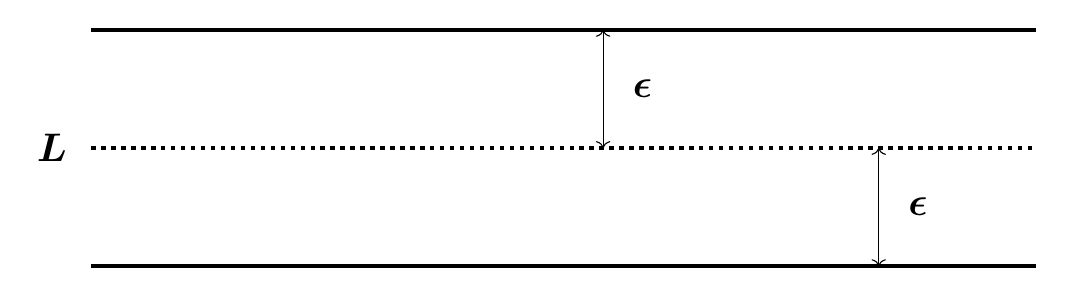
\begin{tikzpicture}

% Draw the two solid lines
\draw[ultra thick] (0,1.5) -- (12,1.5);
\draw[ultra thick] (0,-1.5) -- (12,-1.5);

% Draw the dotted line
\draw[dotted, ultra thick] (0,0) -- (12,0);

% Add the label L
\node at (-0.5,0) {\Large  $\bm{L}$};

% Add the label for 2 epsilon
\draw[<->] (6.5,0) -- (6.5,1.5);
\node at (7,0.75) {\Large $\bm{\epsilon}$};

\draw[<->] (10.,0) -- (10,-1.5);
\node at (10.5,-0.75) {\Large $\bm{\epsilon}$};

\end{tikzpicture}





\newpage

\section{Formulas for the Book Cover}

\begin{enumerate}
\Large
\itemsep4em % Adjust the space between items here



\item $$
e := \lim_{n \to \infty } \left( 1 + \frac{1}{n} \right)^n
$$


\item $$
\int_a^b  dV_{\rm x{\text{-axis}}} = \int_a^b \pi \left( f^2(x) - g^2(x)\right)\,dx
$$

\item $$
\lim_{x \to x_0^-} f(x):=  \lim_{h \to 0^-} f(x_0+h)
$$

\item $$
f(x) \approx f(x_0) + A ( x - x_0) := f(x_0) + \frac{\partial f(x_0)}{\partial x} ( x - x_0)
$$



\item $$
x_{k+1}=x_k - s \left( \nabla f(x_k) \right)
$$

\item
\begin{align*}
\text{Minimize} \quad & f(x)\\
\text{subject to} \quad & g_i(x) = 0, ~ 1\le i \le m,
\end{align*}


\item $$
\frac{d}{dt} \frac{ \partial {\cal L}(q, \dot{q})}{\partial\dot{q}} - \frac{ \partial {\cal L}(q, \dot{q})}{\partial q} = \Gamma
$$

\item $$
\int u \, dv = u\cdot v - \int v \, du
$$

\item $$
\frac{d}{dx} \left[ \int_a^x f(t) \, dt \right] = f(x)
$$

\item $$
e^{A t}:=  \sum_{k=0}^\infty A^k \cdot \frac{t^k}{k!}
$$



\item $$
e^{\im x}:= \cos(x) + \im \sin(x)
$$


\item $$
\bigcap_{i=1}^n \nullspace\left(  J_{g_i}(x_0) \right) \subset   \nullspace\left( J_f(x_0) \right)
$$


\item $$
v(t) = v_0 +  \int_{t_0}^t a(\tau) d\tau
$$

\item $$
\int_{a}^{c} f(x)\, dx =\int_{a}^{b} f(x)\, dx + \int_{b}^{c} f(x)\, dx
$$

\item $$
\nabla \left( f(x) \bullet g(x) \right) = \left[ \frac{\partial g(x)}{\partial x} \right]^\top \cdot  f(x)  + 
\left[ \frac{\partial f(x)}{\partial x} \right]^\top \cdot g(x)
$$

\item $$
S = \int_{t_1}^{t_2} \sqrt{\left(\frac{dx}{dt}\right)^2 + \left(\frac{dy}{dt}\right)^2} \, dt
$$

\end{enumerate}

\newpage
\section{TikZ for Project 3}

\subsection{Decomposed TF for the BallBot}
\bigskip

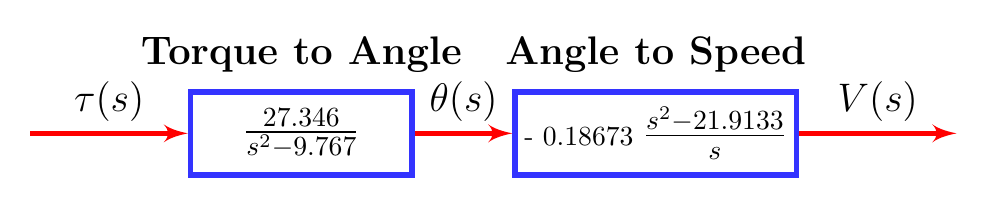
\begin{tikzpicture}[auto, node distance=2cm, >=latex']
 % We define the styles for the blocks and the arrows
 \tikzset{
block/.style = {draw, rectangle, thick, draw=blue!80, line width=2pt, minimum height=3em, minimum width=8em},
line/.style = {draw, -latex', thick, red, line width=2pt},
}

 % Motor torque block
 \node [block] (motor) {\Large $\frac{27.346}{s^2 - 9.767}$ };
 \node [above of=motor,node distance=1cm] (motorlabel) {\textbf{\Large Torque to Angle}};

 % Body orientation block
 \node [block, right of=motor, node distance=4.5cm] (body) {- 0.18673 {\Large $\frac{s^2- 21.9133}{s} $}};
 \node [above of=body,node distance=1cm] (bodylabel) {\textbf{\Large Angle to Speed}};

 % Arrows and labels for input and output
 \draw [line] ([xshift=-2cm]motor.west) -- (motor.west) node[midway, above, black] {\Large $\tau(s)$}; 
 %%node[at start, left, black] {\large Input};
 \draw [line](motor.east) -- (body.west) node[midway, above, black] {\Large $\theta(s)$};
 \draw [line] (body.east) -- ([xshift=2cm]body.east) node[midway, above, black] {\Large $V(s)$};
 %node[at end, right, black] {\large Output};

\end{tikzpicture}

\subsection{First Closed-Loop with Pre-compensator}

\bigskip

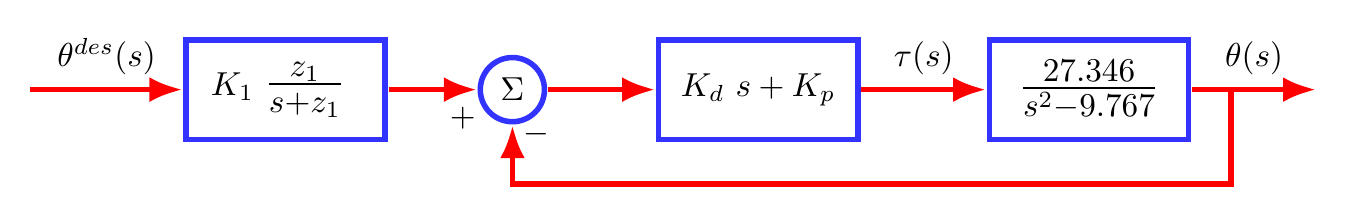
\begin{tikzpicture}[>=Latex, thick, line/.style={draw=red, line width=2pt}, border/.style={draw=blue!80, line width=2pt}, scale=1.2, every node/.style={scale=1.2}]
% Define styles for blocks, sum nodes, input and output
\tikzstyle{block} = [draw, fill=white, rectangle, minimum height=3em, minimum width=6em, border]
\tikzstyle{sum} = [draw, fill=white, circle, node distance=2cm, border]
\tikzstyle{input} = [coordinate]
\tikzstyle{output} = [coordinate]

% Nodes placement
\node [input, name=input] {};
\node [block, right of=input, node distance=2.7cm] (filter) {$K_1$ {\Large  $\frac{z_1}{s + z_1}$ } };
\node [sum, right of=filter, node distance=2.4cm] (sum) {\(\Sigma\)};
\node [block, right of=sum, node distance=2.6cm] (controller) {$K_d~s + K_p$};
\node [block, right of=controller, node distance=3.5cm] (system) {\Large $ \frac{27.346}{s^2 - 9.767 }$};
\node [output, right of=system, node distance=2.4cm] (output) {};

% Draw edges
\draw[line=2pt,->] (input) -- node[above] {$\theta^{des}(s)$} (filter);
\draw[line=2pt,->] (filter) -- node[above] { } (sum);
\draw[line=2pt,->] (sum) -- node[above] {} (controller);
\draw[line=2pt,->] (controller) -- node[above] {$\tau(s)$} (system);
\draw[line=2pt] (system) -- ++(1.5,0) coordinate (feedbackPoint); % Extend line to the right for feedback
\draw[line=2pt,->] (system) -- node[above] {$\theta(s)$} (output); % Continue to output

% Creating a new feedback loop without the Y(s) block
\draw[line=2pt] (feedbackPoint) |- ($(sum)!0.5!(controller)-(0,1cm)$);
\draw[line=2pt,->] ($(sum)!0.5!(controller)-(0,1cm)$) -| node[pos=0.99, right] {$ $} (sum.south);

% Labeling the sum block
\draw (sum.west) ++(-0.15,-0.3) node {$+$};
\draw (sum.south) ++(0.25,-0.1) node {$-$};
\end{tikzpicture}




\subsection{First Closed-Loop with Pre-compensator and an Extra Block that I do not want}

\bigskip

\begin{center}  
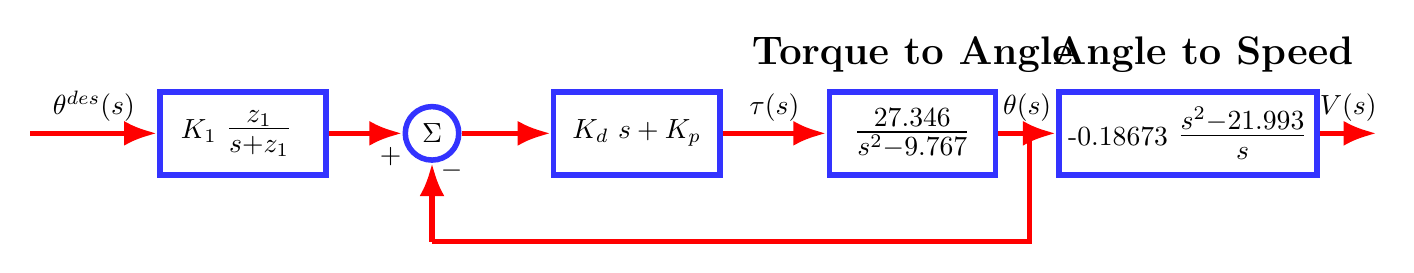
\begin{tikzpicture}[>=Latex, thick, line/.style={draw=red, line width=2pt}, border/.style={draw=blue!80, line width=2pt}, scale=1.0, every node/.style={scale=1.0}]
% Define styles for blocks, sum nodes, input and output
\tikzstyle{block} = [draw, fill=white, rectangle, minimum height=3em, minimum width=6em, border]
\tikzstyle{sum} = [draw, fill=white, circle, node distance=2cm, border]
\tikzstyle{input} = [coordinate]
\tikzstyle{output} = [coordinate]

% Nodes placement
\node [input, name=input] {};
\node [block, right of=input, node distance=2.7cm] (filter) { $K_1$ {\Large $\frac{z_1}{s + z_1}$  } };

\node [sum, right of=filter, node distance=2.4cm] (sum) {\(\Sigma\)};
\node [block, right of=sum, node distance=2.6cm] (controller) {$K_d~ s + K_p$};
\node [block, right of=controller, node distance=3.5cm] (system) {\Large $ \frac{27.346}{s^2 - 9.767 }$};
\node [above of=system,node distance=1cm]{\textbf{\Large Torque to Angle}};

% New block
\node [block, right of=system, node distance=3.5cm] (newblock) {-0.18673 \Large $ \frac{s^2- 21.993}{s}$}; 
 \node [above of=newblock,node distance=1cm] (newblocklabel) {\textbf{\Large ~~Angle to Speed}};

% New output node
\node [output, right of=newblock, node distance=2.4cm] (newoutput) {};

% Draw edges
\draw[line=2pt,->] (input) -- node[above] {$\theta^{des}(s)$} (filter);
\draw[line=2pt,->] (filter) -- node[above] { } (sum);
\draw[line=2pt,->] (sum) -- node[above] {} (controller);
\draw[line=2pt,->] (controller) -- node[above] {$\tau(s)$} (system);
\draw[line=2pt,->] (system) -- node[above] {$\theta(s)$} (newblock);
\draw[line=2pt,->] (newblock) -- node[above] {$V(s)$} (newoutput); % Arrow and label for new block

% Feedback loop
\draw[line=2pt] ($(system.east) + (0.4cm,0)$) |- ($(sum.south) - (0,1cm)$);
\draw[line=2pt,->] ($(sum.south) - (0,1cm)$) -| node[pos=0.99, right] {$ $} (sum.south);

% Labeling the sum block
\draw (sum.west) ++(-0.15,-0.3) node {$+$};
\draw (sum.south) ++(0.25,-0.1) node {$-$};
\end{tikzpicture}
\end{center}


\subsection{Inner-Loop Outer-Loop Control}

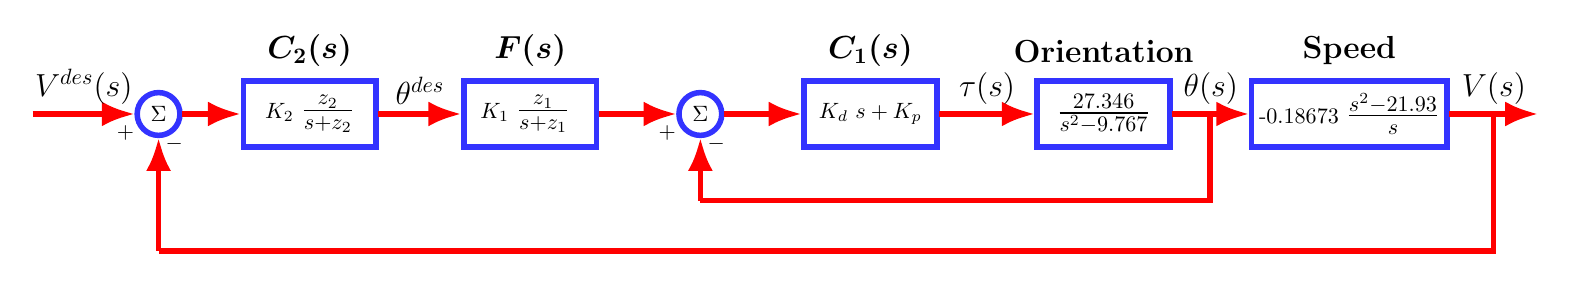
\begin{tikzpicture}[>=Latex, thick, line/.style={draw=red, line width=2pt}, border/.style={draw=blue!80, line width=2pt}, scale=0.8, every node/.style={scale=0.8}]
% Define styles for blocks, sum nodes, input and output
\tikzstyle{block} = [draw, fill=white, rectangle, minimum height=3em, minimum width=6em, border]
\tikzstyle{sum} = [draw, fill=white, circle, node distance=2cm, border]
\tikzstyle{input} = [coordinate]
\tikzstyle{output} = [coordinate]

% Nodes placement
\node [input, name=input] {};
\node [sum, right of=input, node distance=2.0cm] (newsum) {\(\Sigma\)};
\node [block, right of=newsum, node distance=2.4cm] (newblock) {$K_2$ {\Large $  \frac{z_2}{s + z_2}$}};
\node [above of=newblock,node distance=1cm] (C2label) {\textbf{\Large $\bm{C_2(s)}$}};
\node [block, right of=newblock, node distance=3.5cm] (filter) {$K_1$ {\Large  $\frac{z_1}{s + z_1}$ } };
\node [above of=filter,node distance=1cm] (Filterlabel) {\textbf{\Large $\bm{F(s)}$}};
\node [sum, right of=filter, node distance=2.7cm] (sum) {\(\Sigma\)};
\node [block, right of=sum, node distance=2.7cm] (controller) {$K_d~s + K_p$};
\node [above of=controller,node distance=1cm] (C1label) {\textbf{\Large $\bm{C_1(s)}$}};
\node [block, right of=controller, node distance=3.7cm] (system) {\Large $ \frac{27.346}{s^2 - 9.767}$};
\node [above of=system,node distance=1cm] (systemlabel) {\textbf{\Large {\bf Orientation}}};
\node [block, right of=system, node distance=3.9cm] (newblock2) {-0.18673 \Large $ \frac{s^2- 21.93}{s}$};
\node [above of=newblock2,node distance=1cm] (newblock2label) {\textbf{\Large {\bf Speed}}};
\node [output, right of=newblock2, node distance=3.0cm] (output) {};

% Draw edges
\draw[line=2pt,->] (input) -- node[above] {\Large $ V^{des}(s)$} (newsum);
\draw[line=2pt,->] (newsum) -- (newblock);
\draw[line=2pt,->] (newblock) -- node[above] {\Large $\theta^{des}$} (filter);
\draw[line=2pt,->] (filter) -- (sum);
\draw[line=2pt,->] (sum) -- (controller);
\draw[line=2pt,->] (controller) -- node[above] {\Large  $\tau(s)$} (system);
\draw[line=2pt,->] (system) -- node[above] {\Large $\theta(s)$} (newblock2);
\draw[line=2pt,->] (newblock2) -- node[above] {\Large  $V(s)$} (output);

% Feedback loop from system to sum
\draw[line=2pt] (system.east) -- ++(0.6cm,0) |- ($(sum.south)+(0,-1cm)$);
\draw[line=2pt,->] ($(sum.south)+(0,-1cm)$) -| (sum.south);

% Labeling the sum block (existing one)
\draw (sum.west) ++(-0.15,-0.3) node {$+$};
\draw (sum.south) ++(0.25,-0.1) node {$-$};

% Feedback loop from newblock2 to newsum
\draw[line=2pt] (newblock2.east) -- ++(0.7cm,0) |- ($(newsum.south)+(0,-1.8cm)$);
\draw[line=2pt,->] ($(newsum.south)+(0,-1.8cm)$) -| (newsum.south);

% Labeling the new sum block
\draw (newsum.west) ++(-0.15,-0.3) node {$+$};
\draw (newsum.south) ++(0.25,-0.1) node {$-$};
   
\end{tikzpicture}

\subsection{Isolating the controller elements}

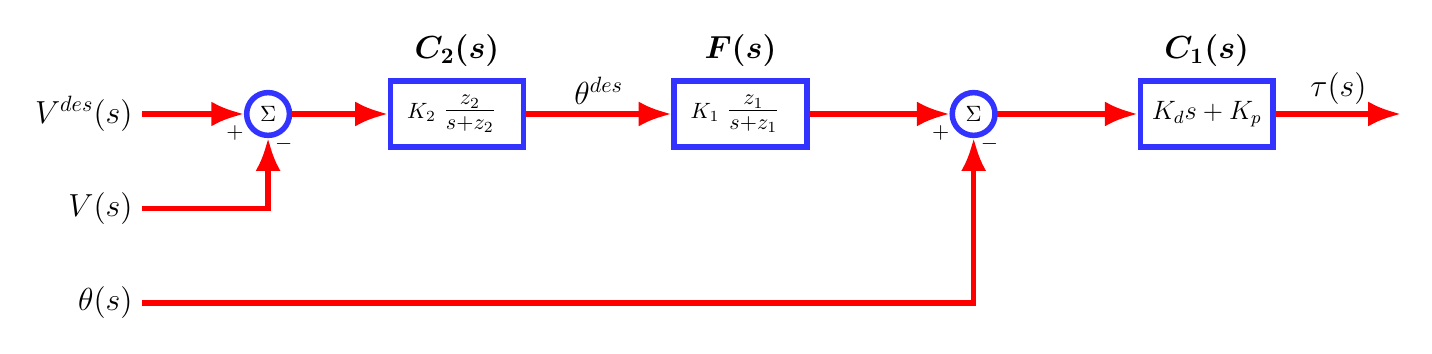
\begin{tikzpicture}
[>=Latex, thick, line/.style={draw=red, line width=2pt}, border/.style={draw=blue!80, 
line width=2pt}, scale=0.8, every node/.style={scale=0.8}]
% Define styles for blocks, sum nodes, input and output
\tikzstyle{block} = [draw, fill=white, rectangle, minimum height=3em, minimum width=6em, border]
\tikzstyle{sum} = [draw, fill=white, circle, node distance=2cm, border]
\tikzstyle{input} = [coordinate]
\tikzstyle{output} = [coordinate]

% Nodes placement
\node [input, name=input] {};
\node [sum, right of=input, node distance=2.0cm] (newsum) {\(\Sigma\)};
\node [block, right of=newsum, node distance=3cm] (newblock) {$K_2$ {\Large $  \frac{z_2}{s+ z_2}$ } };
\node [above of=newblock,node distance=1cm] (C2label) {\textbf{\Large $\bm{C_2(s)}$}};
\node [block, right of=newblock, node distance=4.5cm] (filter) {$K_1$ {\Large  $\frac{z_1}{s + z_1}$ } };
\node [above of=filter,node distance=1cm] (Filterlabel) {\textbf{\Large $\bm{F(s)}$}};
\node [sum, right of=filter, node distance=3.7cm] (sum) {\(\Sigma\)};
\node [block, right of=sum, node distance=3.7cm] (controller) {\large $K_d s + K_p$};
\node [above of=controller,node distance=1cm] (C1label) {\textbf{\Large $\bm{C_1(s)}$}};

% Draw edges
%\draw[line=2pt,->] (input) -- node[above] {\Large $ V^{des}(s)$} (newsum);
\draw[line=2pt,->] (newsum) -- (newblock);
\draw[line=2pt,->] (newblock) -- node[above] {\Large $\theta^{des}$} (filter);
\draw[line=2pt,->] (filter) -- (sum);
\draw[line=2pt,->] (sum) -- (controller);

% Extend a red arrow to the right from the controller block with label
\draw[line=2pt,->] (controller.east) -- ++(2cm,0) node[midway, above] {\Large $\tau(s)$};

\node [input, below of=input, node distance=1.5cm] (input2) {};
\node [input, below of=input, node distance=3.0cm] (input3) {};


% Draw a red line from input2 to the south port of newsum, label in black at the far left
\draw[line=2pt,->,red] (input2) -| node[pos=0, left, black] {\Large $V(s)$} (newsum.south);

% Draw a red line from input3 to the south port of sum, label in black at the far left
\draw[line=2pt,->,red] (input3) -| node[pos=0, left, black] {\Large $\theta(s)$} (sum.south);

% Draw a line from input to newsum with label at the far left
\draw[line=2pt,->] (input) -- node[pos=0, left] {\Large $ V^{des}(s)$} (newsum);


% Labeling the new sum block
\draw (newsum.west) ++(-0.15,-0.3) node {$+$};
\draw (newsum.south) ++(0.25,-0.1) node {$-$};

% Labeling the sum block (existing one)
\draw (sum.west) ++(-0.15,-0.3) node {$+$};
\draw (sum.south) ++(0.25,-0.1) node {$-$};   
\end{tikzpicture}

\end{document}